%!TEX TS-program = xelatex
%!TEX engine = xelatex

\documentclass{standalone}

\usepackage{fontspec}
\setmainfont{Fira Mono}
\usepackage{unicode-math}
\setmathfont[Scale=MatchUppercase]{STIX Two Math}
\setmathrm[Scale=MatchUppercase,
           BoldFont=STIX Two Text Bold]{STIX Two Math}
\setmathtt[Scale=MatchUppercase]{Fira Mono}

\usepackage{tikz}

\begin{document}
  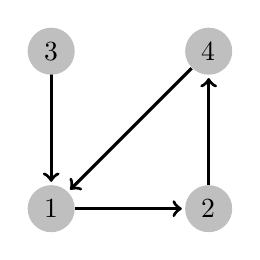
\begin{tikzpicture}[shorten >=1pt]
  \tikzstyle{vertex}=[circle,fill=black!25,minimum size=17pt,inner sep=0pt]

  \path
    (0, 0) node[vertex] (v1) {$1$} --
    (2, 0) node[vertex] (v2) {$2$} --
    (2, 2) node[vertex] (v4) {$4$} -- cycle;

  \foreach \f/\t in {1/2,2/4,4/1}
    \path[draw, very thick, ->]
      (v\f) edge (v\t);

  \path[draw, very thick, ->]
    (0, 2) node[vertex] (v3) {$3$} -- (v1);


  \end{tikzpicture}
\end{document}
